\documentclass[a4paper,12pt,twoside,final]{book}
\usepackage[utf8]{inputenc}
\usepackage[spanish,es-nodecimaldot]{babel} % International, rec. by RAE: http://www.tex-tipografia.com/marca_decimal.html

% COLOR
\usepackage[usenames,dvipsnames,svgnames,table]{xcolor}
% Colores para portada
\definecolor{epsc:oscuro}{HTML}{280091}
 \definecolor{epsc:medio}{HTML}{4C5CC5}
 \definecolor{epsc:claro}{HTML}{3FCFD5}
 \definecolor{epsc:verde}{HTML}{00B299}

 % --- Colores renombrados (sin los dos puntos) ---
\definecolor{epscoscuro}{RGB}{44, 62, 80}  
\definecolor{epscmedio}{RGB}{52, 152, 219} 
\definecolor{epscverde}{RGB}{39, 174, 96}  

\usepackage{tikz}
\usepackage{verbatim}
\usepackage{float}
\usepackage{caption}
\usepackage[hidelinks]{hyperref}
\usetikzlibrary{arrows.meta, positioning}

% UTILs
\usepackage{datetime} % allow formal date format
% "Month, YEAR" date format, in spanish with the month uppercased not interfering other dates
\newcommand\Monthname[1][EMPTY]{
  \ifnum1=#1Enero\else
  \ifnum2=#1Febrero\else
  \ifnum3=#1Marzo\else
  \ifnum4=#1Abril\else
  \ifnum5=#1Mayo\else
  \ifnum6=#1Junio\else
  \ifnum7=#1Julio\else
  \ifnum8=#1Agosto\else
  \ifnum9=#1Septiembre\else
  \ifnum10=#1Octubre\else
  \ifnum11=#1Noviembre\else
  \ifnum12=#1Diciembre\else
  \fi\fi\fi\fi\fi\fi\fi\fi\fi\fi\fi\fi
}
\newdateformat{monthyeardate}{%
  \Monthname[\THEMONTH], \THEYEAR}


% FONTs
\usepackage[T1]{fontenc}
\usepackage{textcomp}           % Needed for new symbols like € ?

\usepackage[scaled]{berasans} % Font for the cover similar to Vera 33
%\renewcommand*\familydefault{\sfdefault}  %% To use as the base font of the document is to be sans serif


% PAGE STYLE
\usepackage[twoside,bindingoffset=0mm,headheight=16pt,margin=25mm]{geometry} 
\usepackage{fancyhdr}
\pagestyle{fancy}
\fancyhf{} % Borra cabeceras y pies actuales

% Configuración para páginas pares (even) e impares (odd)
\fancyhead[LE]{\leftmark}    % Left Even: Capítulo a la izquierda
\fancyhead[RO]{\rightmark}   % Right Odd: Sección a la derecha
\fancyfoot[C]{\thepage}      % Número de página al centro

% Ajustar el ancho de la línea del encabezado (opcional)
\renewcommand{\headrulewidth}{0.4pt}

%Paquete para gestionar la bibliografía
\usepackage[backend=bibtex, style=numeric, sorting=none, maxbibnames=6]{biblatex}

% Carga el fichero de bibliografía
\addbibresource{bib.bib}

% TABLES AND FIGURES
\usepackage{graphicx}
\graphicspath{ {img/} }

\usepackage{titlesec}

% Configuramos el formato de los capítulos:
% [hang] hace que el número y el título estén en la misma línea
\titleformat{\chapter}[hang]
{\normalfont\huge\bfseries} % Estilo del texto (Grande y Negrita)
{\thechapter}               % Solo el número (sin la palabra Capítulo)
{20pt}                      % Espacio entre el número y el título
{\huge}                     % Estilo del título

% Hace que las páginas en blanco entre capítulos no tengan número ni encabezado
\makeatletter
\def\cleardoublepage{\clearpage\if@twoside \ifodd\c@page\else
\hbox{}
\thispagestyle{empty}
\newpage
\if@twocolumn\hbox{}\newpage\fi\fi\fi}
\makeatother
\usepackage[hidelinks]{hyperref}
\begin{document}
\frontmatter

%
% INSTRUCCIONES:
% - Cambia a el escudo de tu titulación comentando y descomentando las líneas correspondientes
% - Cambia todos los textos que están entre '<' y '>' por lo que corresponda en tu proyecto
%


%------------- Cover --------------
\thispagestyle{empty}

% Backgroud images
\begin{tikzpicture}[remember picture, overlay]
  % Top
  \node [anchor=north east, inner sep=0pt]  at (current page.north east)
     {
\includegraphics[height=6cm]{topRightCorner.pdf}};
  % Bottom
  \node [anchor=south west, inner sep=0pt]  at (current page.south west)
     {
\includegraphics[height=6cm]{bottomLeftCorner.pdf}};
  \node (uco) [anchor=south east, inner sep=0pt, xshift=-10mm, yshift=10mm]  at (current page.south east)
        {
\includegraphics[height=2cm]{logoUCO.pdf}};
  \node [anchor=south east, inner sep=0pt, xshift=-10mm]  at (uco.south west)
% ---- Escudo de la titulación correspondiente ----
        {
\includegraphics[height=2cm]{emblema-ing-informatica.pdf}};
%        {
\includegraphics[height=2cm]{emblema-ing-industrial.pdf}};
%        {
\includegraphics[height=2cm]{emblema-ing-tec-industrial.pdf}};
\end{tikzpicture}


\begin{center}
\fontfamily{\sfdefault}\selectfont
\vspace*{2cm}

\vfill
\vfill

\includegraphics[width=12.5cm]{LogotipoEPSC.pdf}
\vfill
\vfill

\large\textbf{\color{epsc:medio}
  TRABAJO FIN DE GRADO
}
\vfill

\Large\textbf{\color{epsc:verde}
  Grado en Ingeniería Informática
}
\vfill
\vfill

\Huge\textbf{\color{epsc:oscuro}
  Diseño y desarrollo de un asistente conversacional educativo para el apoyo al aprendizaje adaptativo
}
\vfill
\vfill

\large{\color{epsc:oscuro}Autor}\\
\textbf{\color{epsc:medio} Rafael David Tortosa Bueno }
\vfill

\large{\color{epsc:oscuro} Director }\\
\textbf{\color{epsc:medio} Dra. Amelia Zafra Gómez }
\vfill



\textbf{\color{epsc:verde} \monthyeardate\today}
\vfill
\vfill
\vspace{2.7cm}
\end{center}


%-------------------------------------------------------------------------------------------------------
\clearpage

\thispagestyle{empty}
\pagecolor{white}

\cleardoublepage
%-------------------------------------------------------------------------------------------------------

%------------- Índices --------------
\pagestyle{empty}
\tableofcontents
\listoffigures
\listoftables

\mainmatter

%------------- Capítulos --------------
\pagestyle{fancy}

\chapter{Introducción y contexto}
\label{cap:introduccion}

La incorporación de la Inteligencia Artificial (IA) en el ámbito educativo ha impulsado el uso de asistentes conversacionales (\textit{chatbots}) como herramienta de apoyo al estudio. Estos sistemas pueden resolver dudas, proporcionar explicaciones y ofrecer recursos de forma inmediata, lo que resulta especialmente útil ante la falta de atención personalizada y la diversidad de ritmos de aprendizaje. Sin embargo, la literatura también señala retos relevantes asociados a su uso (fiabilidad, evaluación, sesgos, ética y privacidad), por lo que su integración debe orientarse a complementar la docencia, fomentar un uso crítico y establecer mecanismos de supervisión y evaluación \cite{Labadze2023}.\\

En particular, en contextos con alta ratio estudiante-profesor, el apoyo conversacional puede actuar como un ``acompañamiento'' entre sesiones presenciales, ayudando a mantener la continuidad del estudio (p.\,ej., resolviendo dudas frecuentes, proponiendo ejercicios de refuerzo o guiando hacia recursos adecuados). Para que este apoyo sea pedagógicamente útil, resulta clave que el asistente no se limite a respuestas genéricas, sino que adapte el tipo de ayuda a las necesidades reales del estudiante y a su nivel de dominio.\\

En paralelo, el \textit{aprendizaje adaptativo} busca ajustar actividades y contenidos en función del desempeño del estudiante, favoreciendo itinerarios formativos más eficaces y personalizados. En esta línea, estudios recientes exploran asistentes educativos con mecanismos de adaptación más avanzados, combinando análisis de interacción, registro de métricas y estrategias de retroalimentación ajustadas al desempeño (e incluso a dimensiones afectivas), con resultados que sugieren mejoras en rendimiento y participación cuando la adaptación se aplica de forma sistemática \cite{Gutierrez2025}.\\

En este contexto se enmarca este Trabajo Fin de Grado, titulado \textit{Diseño y desarrollo de un asistente conversacional educativo para el apoyo al aprendizaje adaptativo}, cuyo propósito es diseñar e implementar un asistente capaz de dar una asistencia dinámica y personalizada según el desempeño de cada estudiante.


\chapter{Objetivos}
\label{cap:objetivos}

El objetivo general de este proyecto es: Diseñar y desarrollar un asistente conversacional orientado al aprendizaje adaptativo, capaz de generar cuestionarios y contenidos conceptuales de forma dinámica, realizar un seguimiento del progreso del estudiante y proporcionar recomendaciones personalizadas que refuercen su aprendizaje.

\section{Objetivos específicos}
\label{sec:obj_especificos}

\begin{enumerate}
    \item \textbf{Módulo de cuestionarios dinámicos:} Desarrollar un módulo para generar preguntas cargadas dinámicamente desde un repositorio estructurado para cada tema, permitiendo que el contenido sea actualizable sin necesidad de modificar el código del asistente.
    \item \textbf{Módulo de repaso de conceptos dinámicos:} Desarrollar un sistema que permita ofrecer repasos de conceptos cargados dinámicamente desde un repositorio estructurado para cada tema, permitiendo que el contenido sea actualizable sin necesidad de modificar el código del asistente.
    \item \textbf{Módulo de seguimiento del progreso del estudiante:} Registrar y almacenar métricas de uso por estudiante (número de sesiones, tiempo de interacción, ejercicios completados, porcentaje de acierto), con el fin de analizar su evolución y facilitar una retroalimentación más precisa.
    \item \textbf{Módulo de recomendaciones:} Diseñar un módulo de recomendación que analice el desempeño del estudiante y sugiera contenidos, repasos o logros obtenidos para reforzar su proceso de aprendizaje de manera personalizada.
\end{enumerate}

\chapter{Antecedentes}
\label{cap:antecedentes}

Este Trabajo Fin de Grado se plantea como una \textbf{continuación y evolución} de un desarrollo previo de un chatbot educativo orientado a la docencia universitaria\footnote{I. A. Ruiz Martin-Romo, \textit{Diseño y desarrollo de un Chatbot como recurso para la docencia (Manual técnico)}, Universidad de Córdoba, junio de 2022.}. En dicho trabajo se implementó un asistente conversacional para la asignatura de Redes de la Universidad de Córdoba, con funciones de consulta de información administrativa (horarios, tutorías, profesorado) y apoyo al estudio mediante repasos, cuestionarios y ejercicios con retroalimentación.\\

No obstante, aquel sistema presentaba limitaciones relevantes para un enfoque adaptativo: el número de conceptos y ejercicios por tema era reducido y fijo, la actualización del contenido resultaba costosa al depender de una estructura poco flexible, no se mantenía un registro sistemático de interacciones y rendimiento por estudiante y no existía un módulo de recomendación que guiara el refuerzo en función del historial. Este proyecto tiene como finalidad evolucionar el sistema hacia una herramienta de acompañamiento que fomente el aprendizaje adaptativo, la motivación y la personalización de la experiencia educativa, apoyándose en repositorios dinámicos de contenido, métricas de progreso y recomendaciones.\\

\section{Plataformas y marcos de desarrollo de chatbots}
\label{sec:plataformas}

En el ámbito de los asistentes conversacionales existen diversas alternativas para su construcción, desde servicios comerciales en la nube hasta soluciones \textit{open-source}. Entre las plataformas comerciales más utilizadas se encuentran IBM Watson Assistant \cite{ibmWatsonAssistant}, Microsoft Azure Bot Service \cite{azureBotService} o Amazon Lex \cite{amazonLex}, que ofrecen integración con servicios cloud y despliegues gestionados. En paralelo, librerías y marcos generalistas como TensorFlow \cite{tensorflow} posibilitan construir modelos de PLN\footnote{Procesamiento del Lenguaje Natural} a medida, si bien suelen requerir mayor esfuerzo de ingeniería para completar la gestión del diálogo, la integración con canales y el mantenimiento del sistema. \\


En el dominio educativo han ganado relevancia marcos \textit{open-source} que permiten un mayor control y personalización del comportamiento del bot, especialmente cuando se requiere adaptar el flujo conversacional y conectarlo con recursos propios de la asignatura o la institución. Dentro de estas alternativas destaca Rasa \cite{rasaDocs}, un marco de IA conversacional que proporciona componentes para (i) comprensión del lenguaje natural (clasificación de intenciones y extracción de entidades) y (ii) gestión del diálogo mediante predicción de la siguiente acción, facilitando además la integración mediante acciones personalizadas y el manejo del estado conversacional.\\

Distintos trabajos han utilizado Rasa para construir chatbots educativos o institucionales. Por ejemplo, Supreetha y Sandhya describen la implementación de un chatbot educativo con Rasa, destacando el flujo de entrenamiento y despliegue \cite{Supreetha2022}; Badgujar \textit{et al.} presentan un bot educativo basado en Rasa y discuten su estructura modular \cite{Badgujar2023}; y Kale \textit{et al.} abordan un chatbot conversacional para facilitación educativa, enfatizando escenarios de uso y despliegue \cite{Kale2025}. Estas aportaciones respaldan la idoneidad de Rasa para asistentes entrenables y extensibles en contextos docentes.

\section{Chatbots educativos y evolución hacia la personalización}
\label{sec:personalizacion}

El uso de chatbots en educación se ha orientado a múltiples objetivos: apoyo al aprendizaje de contenidos, asistencia administrativa, evaluación y motivación del estudiante. La investigación reciente muestra que los chatbots pueden aportar beneficios como apoyo al estudio y experiencias de aprendizaje más personalizadas; no obstante, también se señalan desafíos relevantes en fiabilidad, precisión y consideraciones éticas, por lo que se recomienda incorporar estrategias de evaluación y uso responsable \cite{Labadze2023}. \\

En la línea de la personalización, estudios recientes exploran asistentes educativos con mecanismos de adaptación más avanzados, combinando análisis de interacción, registro de métricas y estrategias de retroalimentación ajustadas al desempeño (e incluso a dimensiones afectivas), con resultados que sugieren mejoras en rendimiento y participación cuando la adaptación se aplica de forma sistemática \cite{Gutierrez2025}. Asimismo, en trabajos basados en Rasa se plantea como extensión natural la incorporación de módulos de seguimiento del progreso y sistemas de recomendación para reforzar el aprendizaje y orientar al estudiante en función de su historial de interacción \cite{Supreetha2022}.

\chapter{Análisis del problema}
\label{cap:analisis_problema}
En el presente apartado se expondrán las limitaciones de la anterior versión de este proyecto, ya mencionado en el apartado \ref{cap:antecedentes}. Además, se definirán los problemas real y técnico para la correcta comprensión de los desafíos que motivan el desarrollo de este trabajo.

\section{Definición del problema real}
\label{sec:def_problema}
El sistema anterior, aunque era funcional para el alumnado como herramienta de consulta, presentaba una gran limitación para el profesorado debido a su codificación totalmente estática. De forma que si se quiere añadir algún concepto, cuestionario o incluso modificar los horarios para el próximo año, se debe cambiar del núcleo del bot en el que están las reglas e intenciones \textit{hardcodeadas}.\\

Con respecto al módulo de cuestionarios y ejercicios prácticos, el bot solo acepta respuestas como \texttt{A1} o \texttt{A3}, siendo estas las opciones a de las preguntas 1 y 3. Este comportamiento es debido a que, como ya se mencionó anteriormente, las intenciones de estas preguntas están \textit{hardcodeadas} y, por tanto, el sistema no permite tener intenciones repetidas como serían \texttt{A} o \texttt{B}.\\

Por otro lado, el sistema de retroalimentación presenta una restricción funcional significativa al solo procesar la información del propio núcleo sin tener en cuenta el usuario ni sus interacciones pasadas con el bot. Asimismo, al no existir ningún tipo de registro de actividad, el sistema es incapaz de establecer indicadores de trazabilidad del alumno, lo cual imposibilita al profesorado una monitorización del aprendizaje efectiva.
\begin{comment}
\section{Requisitos Funcionales (RF)}

\subsection{Módulos de Contenido Dinámico}
\begin{itemize}
    \item \textbf{RF-01 Carga dinámica de activos pedagógicos:} El sistema deberá recuperar las preguntas de los cuestionarios y los conceptos de repaso desde un repositorio estructurado externo.
    \item \textbf{RF-02 Desacoplamiento de contenido y lógica:} La actualización de los materiales de estudio no deberá requerir modificaciones en el código fuente del asistente ni reinicios del servicio.
    \item \textbf{RF-03 Organización temática:} El sistema deberá filtrar los contenidos dinámicos según el identificador del tema o módulo seleccionado por el usuario.
\end{itemize}

\subsection{Módulo de Seguimiento y Persistencia}
\begin{itemize}
    \item \textbf{RF-04 Gestión de identidad y sesiones:} El sistema deberá identificar a cada estudiante de forma unívoca y registrar el inicio y cierre de sus sesiones de interacción.
    \item \textbf{RF-05 Almacenamiento en base de datos SQL:} Se implementará un esquema relacional para registrar métricas de uso, incluyendo tiempos de respuesta, ejercicios completados y tasas de éxito.
    \item \textbf{RF-06 Histórico de interacciones:} El sistema deberá permitir la recuperación de interacciones pasadas para contextualizar la experiencia del usuario.
\end{itemize}

\subsection{Módulo de Personalización}
\begin{itemize}
    \item \textbf{RF-07 Motor de recomendaciones proactivas:} El sistema deberá analizar el desempeño histórico almacenado en la base de datos SQL para sugerir contenidos específicos de refuerzo.
    %\item \textbf{RF-08 Sistema de gamificación y logros:} El sistema verificará el cumplimiento de hitos pedagógicos y registrará la obtención de logros en el perfil del estudiante.
\end{itemize}

\section{Requisitos No Funcionales (RNF)}
\begin{itemize}
    \item \textbf{RNF-01 Integridad de datos:} La base de datos SQL deberá garantizar la consistencia de la información del progreso del alumno mediante transacciones seguras.
    \item \textbf{RNF-02 Trazabilidad pedagógica:} El sistema debe permitir reconstruir la evolución del aprendizaje del alumno para facilitar la labor de monitorización del profesorado.
    \item \textbf{RNF-03 Escalabilidad:} El repositorio estructurado debe ser capaz de crecer en volumen de datos sin comprometer la latencia de respuesta del bot.
    \item \textbf{RNF-04 Disponibilidad para supervisión:} Los datos de seguimiento deberán estar estructurados de tal forma que permitan su posterior visualización mediante cuadros de mando para los docentes.
\end{itemize}
\end{comment}

\section{Definición del problema técnico}
Desde una perspectiva de ingeniería, la definición del problema se abordará mediante la metodología \textbf{PDS}\footnote{Product Design Specification}. Esta técnica permite desglosar el problema técnico en los parámetros detallados a continuación:
\subsection{Funcionamiento}

El funcionamiento del asistente se basa en un ciclo de interacción dinámico y centrado en el estudiante, estructurado en tres niveles operativos fundamentales:

\subsubsection*{A. Interacción y Comprensión (Capa de Diálogo)}
El sistema opera mediante un motor de procesamiento de lenguaje natural (NLP) que permite una comunicación bidireccional fluida. A diferencia de versiones anteriores, el flujo no es estrictamente lineal, permitiendo al asistente:
\begin{itemize}
    \item \textbf{Identificar intenciones:} Diferenciar con precisión entre consultas administrativas (tutorías, aulas, fechas de entrega) y peticiones de carácter pedagógico (repaso de conceptos o realización de cuestionarios).
    \item \textbf{Gestión del estado de la conversación:} Mantener el hilo de la interacción mediante el uso de memoria a corto plazo (\textit{slots}), lo que permite al sistema conocer en qué tema o módulo se encuentra el alumno sin que este deba especificarlo en cada mensaje, facilitando una experiencia más natural.
\end{itemize}

\subsubsection*{B. Suministro Dinámico de Contenidos (Capa de Datos)}
El núcleo del avance técnico reside en el desacoplamiento entre la lógica del bot y el material educativo. El proceso operativo ante una solicitud de estudio sigue estos pasos:
\begin{enumerate}
    \item El sistema realiza una consulta a un \textbf{repositorio estructurado externo} (fuera del código fuente del bot).
    \item Se filtran los activos pedagógicos (preguntas, respuestas y explicaciones) en función del identificador del tema solicitado.
    \item Se genera la interfaz de respuesta de forma dinámica, lo que permite al profesorado actualizar el material educativo de manera instantánea sin necesidad de modificar el código ni reiniciar los servicios del asistente.
\end{enumerate}

\subsubsection*{C. Lógica Adaptativa y Seguimiento (Capa de Inteligencia)}
\text{\huge REVISAR}\\
Esta versión introduce un componente de persistencia que transforma el funcionamiento tradicionalmente reactivo en uno proactivo y personalizado:
\begin{itemize}
    \item \textbf{Registro en tiempo real:} Cada interacción y respuesta del alumno se registra en una base de datos relacional (SQL) vinculada a su identificador unívoco, garantizando la trazabilidad del aprendizaje.
    \item \textbf{Evaluación y Retroalimentación:} Tras la finalización de una actividad, el sistema no solo devuelve una corrección inmediata, sino que procesa el desempeño en comparación con el historial del usuario.
    \item \textbf{Motor de Recomendación:} Basándose en el análisis de aciertos y errores, el bot altera su comportamiento para sugerir refuerzos específicos en las áreas donde se detecta debilidad o proponer logros para incentivar la motivación del estudiante.
\end{itemize}

\subsection{Entorno}

El entorno del proyecto se define desde diversas perspectivas técnicas que garantizan el desarrollo, la ejecución y la accesibilidad del asistente:

\begin{itemize}
    \item \textbf{Entorno de desarrollo y programación:} La implementación del sistema se basa íntegramente en el lenguaje de programación \textbf{Python}, seleccionado por su madurez en el ámbito de la Inteligencia Artificial y su ecosistema de librerías especializadas. Como núcleo conversacional se utiliza el marco de trabajo (\textit{framework}) de código abierto \textbf{Rasa}, que proporciona las herramientas necesarias para la gestión de NLU\footnote{\textbf{Natural Language Understanding} o Comprensión del Lenguaje Natural} y diálogos.
    
    \item \textbf{Entorno de ejecución (Software):} El sistema se despliega mediante la tecnología de \textbf{contenedores Docker}, lo que permite aislar los componentes principales (Rasa Server, Action Server y Base de datos) y asegurar su funcionamiento independientemente del sistema \textit{host}. Internamente, las imágenes de Rasa utilizan Python (versión 3.10.x) sobre entornos GNU/Linux.
    
    \item \textbf{Entorno de persistencia:} El sistema requiere un motor de base de datos relacional \textbf{PostgreSQL} para el almacenamiento estructurado de la información del estudiante, profesorado, conceptos, ejercicios y métricas de seguimiento.
    
    \item \textbf{Entorno de usuario y despliegue:} La interfaz de interacción para el estudiante es la plataforma de mensajería \textbf{Telegram}. Se ha seleccionado este canal por su accesibilidad multiplataforma y su capacidad para ofrecer un entorno de comunicación privado. Además, se emplea la herramienta \textbf{Ngrok} para la exposición segura del puerto local del servidor mediante túneles HTTPS, conectándolo con los \textit{webhooks} de Telegram.
\end{itemize}

\subsection{Vida esperada}

La vida útil de este asistente conversacional no viene determinada por el desgaste físico, sino por la vigencia de sus componentes software y su relevancia académica.\\

Por un lado, la \textbf{obsolescencia del software} está ligada a las actualizaciones de las librerías de terceros, especialmente el framework Rasa y las API\footnote{Application Programming Interface} de Telegram. Dado que el ecosistema de la Inteligencia Artificial evoluciona rápidamente, resulta conveniente llevar a cabo revisiones periódicas para adaptar el código a las nuevas versiones de los modelos de lenguaje y protocolos de seguridad.\\

Por otro lado, desde la perspectiva del \textbf{contenido educativo}, la vida esperada es mucho mayor gracias a la arquitectura dinámica implementada. Al estar el conocimiento desacoplado de la lógica del bot, los docentes pueden actualizar los temarios de la asignatura de forma indefinida sin que el sistema quede obsoleto. El asistente seguirá siendo útil mientras la metodología de aprendizaje adaptativo y los planes de estudio de la titulación mantengan su estructura actual.\\

Finalmente, la escalabilidad del diseño permite que, una vez finalizado este ciclo de vida inicial, el bot pueda servir como base para futuras evoluciones, asegurando que el esfuerzo de desarrollo tenga un impacto duradero en la institución.

\subsection{Ciclo de mantenimiento}

El mantenimiento del sistema abarca actuaciones correctivas y evolutivas. Estas incluyen la actualización periódica de las dependencias del software (Rasa, PostgreSQL, librerías de Python), la revisión de compatibilidad ante cambios en las políticas de la API de Telegram, y el monitoreo del rendimiento de la base de datos. Gracias a la contenedorización con Docker, las actualizaciones del entorno de ejecución se simplifican significativamente, permitiendo modificar las versiones de las imágenes base sin alterar la configuración del servidor físico.

\subsection{Competencia}

Aunque existen otros asistentes educativos integrados en plataformas comerciales de aprendizaje (LMS\footnote{Learning Management System}) o chatbots genéricos impulsados por grandes modelos de lenguaje (LLM\footnote{Large Language Model}), la principal ventaja competitiva de este proyecto radica en su \textbf{especialización y soberanía de datos}. El asistente adapta el modelo pedagógico propio de la asignatura sin depender de APIs de pago externas que procesen la información de los estudiantes. Asimismo, se integra de manera directa en una aplicación de uso diario como Telegram, eliminando barreras de adopción y mejorando la cercanía con el alumno.

\subsection{Aspecto externo}

La interfaz visible del sistema es la propia aplicación cliente de Telegram (disponible en formato móvil, escritorio y web). Su aspecto externo corresponde al de un chat convencional, donde el bot interactúa haciendo uso de elementos visuales nativos como botones integrados (\textit{inline keyboards}), comandos de menú (\texttt{/start}) y respuestas enriquecidas con formato (negritas, cursivas, listas o enlaces). Esto garantiza una experiencia de usuario familiar, moderna e intuitiva sin necesidad de desarrollar ni instalar aplicaciones adicionales.

\subsection{Estandarización}

El proyecto se rige por estándares de la industria del desarrollo de software. Emplea contenedores Docker como estándar de facto para el despliegue de aplicaciones; utiliza formatos estandarizados de intercambio de datos como YAML (para la configuración de Rasa) y JSON (para las comunicaciones web); y se apoya en SQL estándar para las operaciones con la base de datos. A nivel de código, la programación en Python respeta las guías de estilo PEP-8, favoreciendo su legibilidad y posterior mantenimiento por parte de la comunidad universitaria.

\subsection{Calidad y fiabilidad}

La fiabilidad del sistema se sustenta en el uso de tecnologías ampliamente testeadas como Rasa y PostgreSQL. A nivel operativo, se han implementado mecanismos de recuperación como políticas de reinicio automático de los contenedores para hacer frente a caídas inesperadas del servicio. En el código del servidor de acciones (\textit{Action Server}), se han incorporado bloques de control de excepciones (\texttt{try/except}) y gestores de contexto (with) que evitan interrupciones críticas en el flujo conversacional, informando al usuario en caso de fallos temporales de conexión con la base de datos y se encargan de abrir y cerrar la conexión con la base de datos automáticamente, respectivamente.

\subsection{Programa de tareas}

Para la consecución de los objetivos planteados, el trabajo se ha estructurado en las siguientes fases principales:
\begin{enumerate}
    \item Análisis de requisitos y evaluación de las limitaciones del sistema predecesor.
    \item Diseño de la nueva arquitectura de despliegue (Rasa 3.x, Docker, PostgreSQL, Ngrok).
    \item Diseño de la base de datos y migración de esquemas.
    \item Implementación de los módulos lógicos (acciones personalizadas) para la gestión del contenido dinámico y el seguimiento del alumno.
    \item Estudio y creación del módulo de recomendación (MLP\footnote{Multi-Layer Perceptron}).
    \item Fases de pruebas de integración y validación del sistema final.
    \item Redacción y estructuración de la memoria del proyecto.
\end{enumerate}

\subsection{Pruebas}

Se ha diseñado una estrategia de validación en varios niveles. A nivel conversacional, se emplean pruebas de flujo (\textit{test stories} y \textit{rules}) propias del entorno Rasa para certificar que el asistente recorre adecuadamente los caminos conversacionales estipulados sin bloqueos. A nivel de sistema, se realizan pruebas de extremo a extremo (\textit{end-to-end}) interactuando directamente desde la aplicación de Telegram, lo que permite verificar la integración completa entre los mensajes del usuario, el procesamiento de Rasa, la ejecución de las acciones en Python y la persistencia de datos en PostgreSQL.

\subsection{Seguridad}

La seguridad se ha abordado de forma integral en el diseño arquitectónico:
\begin{itemize}
    \item \textbf{Aislamiento:} El uso de contenedores restringe el acceso de los servicios al sistema de archivos de la máquina anfitriona.
    \item \textbf{Gestión de credenciales:} Se emplean variables de entorno (mediante archivos \texttt{.env}) para proteger tokens de acceso, contraseñas de bases de datos y configuraciones sensibles, evitando su exposición en repositorios de código.
    \item \textbf{Comunicaciones seguras:} La conexión entre los servidores de Telegram y el entorno local se cifra mediante un túnel HTTPS proporcionado por Ngrok, garantizando la confidencialidad de los datos en tránsito.
    \item \textbf{Privacidad de datos:} Telegram garantiza el cifrado y protección de los mensajes. Adicionalmente, el sistema interno solo almacena el identificador numérico de Telegram del usuario, vinculándolo estrictamente con los datos de progreso académico, respetando el principio de minimización de datos.
\end{itemize}

\section{Requisitos Funcionales (RF)}

\subsection{Módulos de Contenido Dinámico}
\begin{itemize}
    \item \textbf{RF-01 Carga dinámica de activos pedagógicos:} El sistema deberá recuperar las preguntas de los cuestionarios y los conceptos de repaso desde un repositorio estructurado externo.
    \item \textbf{RF-02 Desacoplamiento de contenido y lógica:} La actualización de los materiales de estudio no deberá requerir modificaciones en el código fuente del asistente ni reinicios del servicio.
    \item \textbf{RF-03 Organización temática:} El sistema deberá filtrar los contenidos dinámicos según el identificador del tema o módulo seleccionado por el usuario.
\end{itemize}

\subsection{Módulo de Seguimiento y Persistencia}
\begin{itemize}
    \item \textbf{RF-04 Gestión de identidad y sesiones:} El sistema deberá identificar a cada estudiante de forma unívoca y registrar las sesiones de estudio del alumno (cuestionarios / conceptos).
    \item \textbf{RF-05 Almacenamiento en base de datos SQL:} Se implementará un esquema relacional para registrar métricas de uso, incluyendo tiempos de respuesta, ejercicios completados y tasas de éxito.
    \item \textbf{RF-06 Histórico de interacciones:} El sistema deberá permitir la recuperación de interacciones pasadas para contextualizar la experiencia del usuario.
\end{itemize}

\subsection{Módulo de Personalización}
\begin{itemize}
    \item \textbf{RF-07 Motor de recomendaciones proactivas:} El sistema deberá analizar el desempeño histórico almacenado en la base de datos SQL para sugerir contenidos específicos de refuerzo.
    %\item \textbf{RF-08 Sistema de gamificación y logros:} El sistema verificará el cumplimiento de hitos pedagógicos y registrará la obtención de logros en el perfil del estudiante.
\end{itemize}

\section{Requisitos No Funcionales (RNF)}
\begin{itemize}
    \item \textbf{RNF-01 Integridad de datos:} La base de datos SQL deberá garantizar la consistencia de la información del progreso del alumno mediante transacciones seguras.
    \item \textbf{RNF-02 Trazabilidad pedagógica:} El sistema debe permitir reconstruir la evolución del aprendizaje del alumno para facilitar la labor de monitorización del profesorado.
    \item \textbf{RNF-03 Escalabilidad:} El repositorio estructurado debe ser capaz de crecer en volumen de datos sin comprometer la latencia de respuesta del bot.
\end{itemize}

\chapter{Diseño}
\section{Diseño Arquitectónico y de Despliegue}
\label{sec:diseno_arquitectonico}

El sistema propuesto difiere con la versión anterior del sistema aportando una implementación del software basada en servicios independientes, aislados y gestionados a través de contenedores de Docker. Para dotar de consistencia técnica y automatizar el ciclo de vida del asistente, el entorno de ejecución se orquesta sobre una infraestructura de red virtualizada propia de la plataforma \textit{Docker}, denominada \texttt{rasa-network}, que intercomunica los diferentes servicios de manera nativa sin exponer puertos innecesarios de cara al exterior.

\begin{figure}[H]
    \centering
    \includegraphics[width=1\textwidth]{img/Vista_Despliegue.png}
    \caption{Diagrama de arquitectura, topología de red virtualizada y flujo de automatización del asistente educativo.}
    \label{fig:arquitectura_sistema}
\end{figure}

El proceso de despliegue automatizado y la posterior gestión conversacional se dividen técnicamente en cuatro capas funcionales, implementadas mediante contenedores específicos descritos a continuación:
\newpage

\begin{enumerate}
    \item \textbf{Capa de Almacenamiento (\texttt{postgres\_db}):} Consiste en un contenedor con la imagen oficial de \textit{PostgreSQL 15}. Este componente expone internamente el puerto $5432$ y utiliza un volumen persistente de datos llamado \texttt{postgres\_data} vinculado al directorio interno \texttt{/var/lib/postgresql/data}. En el momento del primer despliegue, el contenedor asocia de manera automática un script de inicialización estructurado (\texttt{script\_bbdd.sql}) mapeado directamente sobre el directorio de arranque automático de la imagen (\texttt{/docker-entrypoint-initdb.d/init.sql}).
    
    \item \textbf{Capa de Lógica de Negocio y Extensibilidad (\texttt{rasa\_action\_server}):} Ejecuta un contenedor con la imagen SDK de Rasa (\texttt{rasa/rasa-sdk:latest}) que expone el puerto estándar $5055$. Su inicialización requiere la importación de las variables de entorno correspondientes a la base de datos relacional (\texttt{DB\_HOST}, \texttt{DB\_USER}, \texttt{DB\_PASSWORD} y \texttt{DB\_NAME}). El arranque del servicio compila e instala en tiempo de ejecución las librerías necesarias para la conexión con la base de datos y el motor de recomendación (\texttt{psycopg2-binary}, \texttt{scikit-learn}, \texttt{numpy} y \texttt{joblib}), invocando el comando de arranque del servidor de acciones en el paquete de Python \texttt{actions}.
    
    \item \textbf{Capa de exposición a Internet y Túnel (\texttt{ngrok}):} Implementa una imagen de \textit{Ngrok} que se integra dentro de la red virtual de Docker. Su función es interceptar el tráfico local del servidor principal y redirigirlo a través de una pasarela segura cifrada bajo el protocolo HTTPS. El contenedor opera de manera síncrona interpretando un archivo de configuración local (\texttt{ngrok.yml}) y vinculando el subdominio generado directamente hacia la interfaz interna del servidor de procesamiento conversacional (\texttt{rasa\_server:5005}).
    
    \item \textbf{Capa de Inteligencia Conversacional y Procesamiento NLU (\texttt{rasa\_server}):} Contiene el núcleo de procesamiento del lenguaje natural del asistente. Se despliega mediante la imagen \texttt{rasa/rasa:latest-full} mapeando el directorio de trabajo sobre la ruta raíz del contenedor (\texttt{/app}). En lugar de instanciar la inicialización tradicional de la herramienta de línea de comandos, el contenedor sobreescribe su punto de entrada (\textit{entrypoint}) para ejecutar de manera exclusiva un script estructurado de orquestación en lenguaje Python (\texttt{docker\_entrypoint.py}).
\end{enumerate}

\subsection{Automatización del Despliegue y Ciclo de Sincronización de Componentes}
Con el propósito de mitigar la necesidad de una supervisión constante y asegurar un entorno predecible, la cohesión del sistema se delega en un flujo autónomo de automatización. Este proceso se despliega en dos fases críticas:

\subsubsection{Inicialización de la Red y Contenedores Base}
A través del script \texttt{run\_with\_docker.sh}, el sistema carga el fichero de variables de entorno (\texttt{.env}) y exporta las credenciales requeridas. Posteriormente, inicializa de manera secuencial los contenedores de almacenamiento (\texttt{postgres\_db}), el servidor de lógica personalizada (\texttt{rasa\_action\_server}) y el túnel de comunicación (\texttt{ngrok}). De este modo, la red queda preparada antes de dar control al contenedor de procesado conversacional.

\subsubsection{Orquestación Dinámica del Punto de Entrada}
Una vez que el contenedor \texttt{rasa\_server} entra en ejecución, el script de control \texttt{docker\_entrypoint.py} realiza los siguientes pasos:
\begin{itemize}
    \item \textbf{Sondeo de Disponibilidad de Red:} El script interroga mediante peticiones HTTP internas empleando la librería estándar \texttt{urllib.request} la API local de Ngrok (\texttt{http://ngrok:4040/api/tunnels}) en un ciclo limitado a quince iteraciones. El bucle se mantiene activo hasta recuperar de manera segura la cadena de texto correspondiente a la URL pública.
    
    \item \textbf{Modificación del Fichero de Credenciales:} Una vez que el script consigue la dirección web pública y segura de \textit{Ngrok}, abre y lee el archivo \texttt{/app/credentials.yml}. Su objetivo es localizar la sección dedicada a la configuración de \texttt{telegram:}. Cuando la encuentra, el script modifica de forma exacta la línea \texttt{webhook\_url:} para añadirle la nueva URL pública junto al sufijo que Rasa necesita por defecto (\texttt{/webhooks/telegram/webhook}). En ese mismo momento, aprovecha para rellenar de manera automática los campos de autenticación (\texttt{access\_token:}) y de verificación (\texttt{verify:}) utilizando los tokens y contraseñas que previamente se habían cargado de forma segura en las variables de entorno del sistema.
    
    \item \textbf{Registro Remoto de Webhook:} Una vez que el archivo de credenciales está listo, el script se conecta directamente con los servidores de Telegram. Para que el alumnado pueda comunicarse con el bot por Telegram, se hace una petición POST a la API oficial (\texttt{https://api.telegram.org/bot<token>/setWebhook}), para así registrar la nueva dirección de \textit{Ngrok}. De esta forma, el puente de comunicación queda registrado de manera definitiva.
    
    \item \textbf{Entrenamiento y Lanzamiento de Servicios:} Por último, el script entrena el modelo de procesamiento conversacional mediante el comando \texttt{rasa train} y transfiere el control del proceso principal de ejecución al servicio conversacional de Rasa utilizando una llamada nativa al sistema operativo (\texttt{os.execvp}), habilitando la API interna, la configuración en modo depuración (\texttt{--debug}) y enlazando los puertos de escucha finales.
\end{itemize}
\text{\Huge Repasar a partir de aquí}
\section{Diseño de la Base de Datos}
\label{sec:diseno_datos}

Para solucionar de forma definitiva la rigidez conceptual y el acoplamiento de datos identificados en la problemática técnica, se ha diseñado un esquema relacional normalizado sobre el motor de base de datos \textit{PostgreSQL 15}. La finalidad primordial de este diseño es desacoplar por completo el conocimiento educativo de la programación del asistente conversacional, permitiendo que el \textit{Action Server} realice consultas SQL dinámicas basadas en los parámetros contextuales de la conversación. \\

El repositorio de persistencia se articula técnicamente mediante una jerarquía de dependencias estructurada en cuatro niveles operativos, lo que optimiza las restricciones de integridad transaccional frente a operaciones de actualización o borrado en cascada.

\begin{figure}[H]
    \centering
    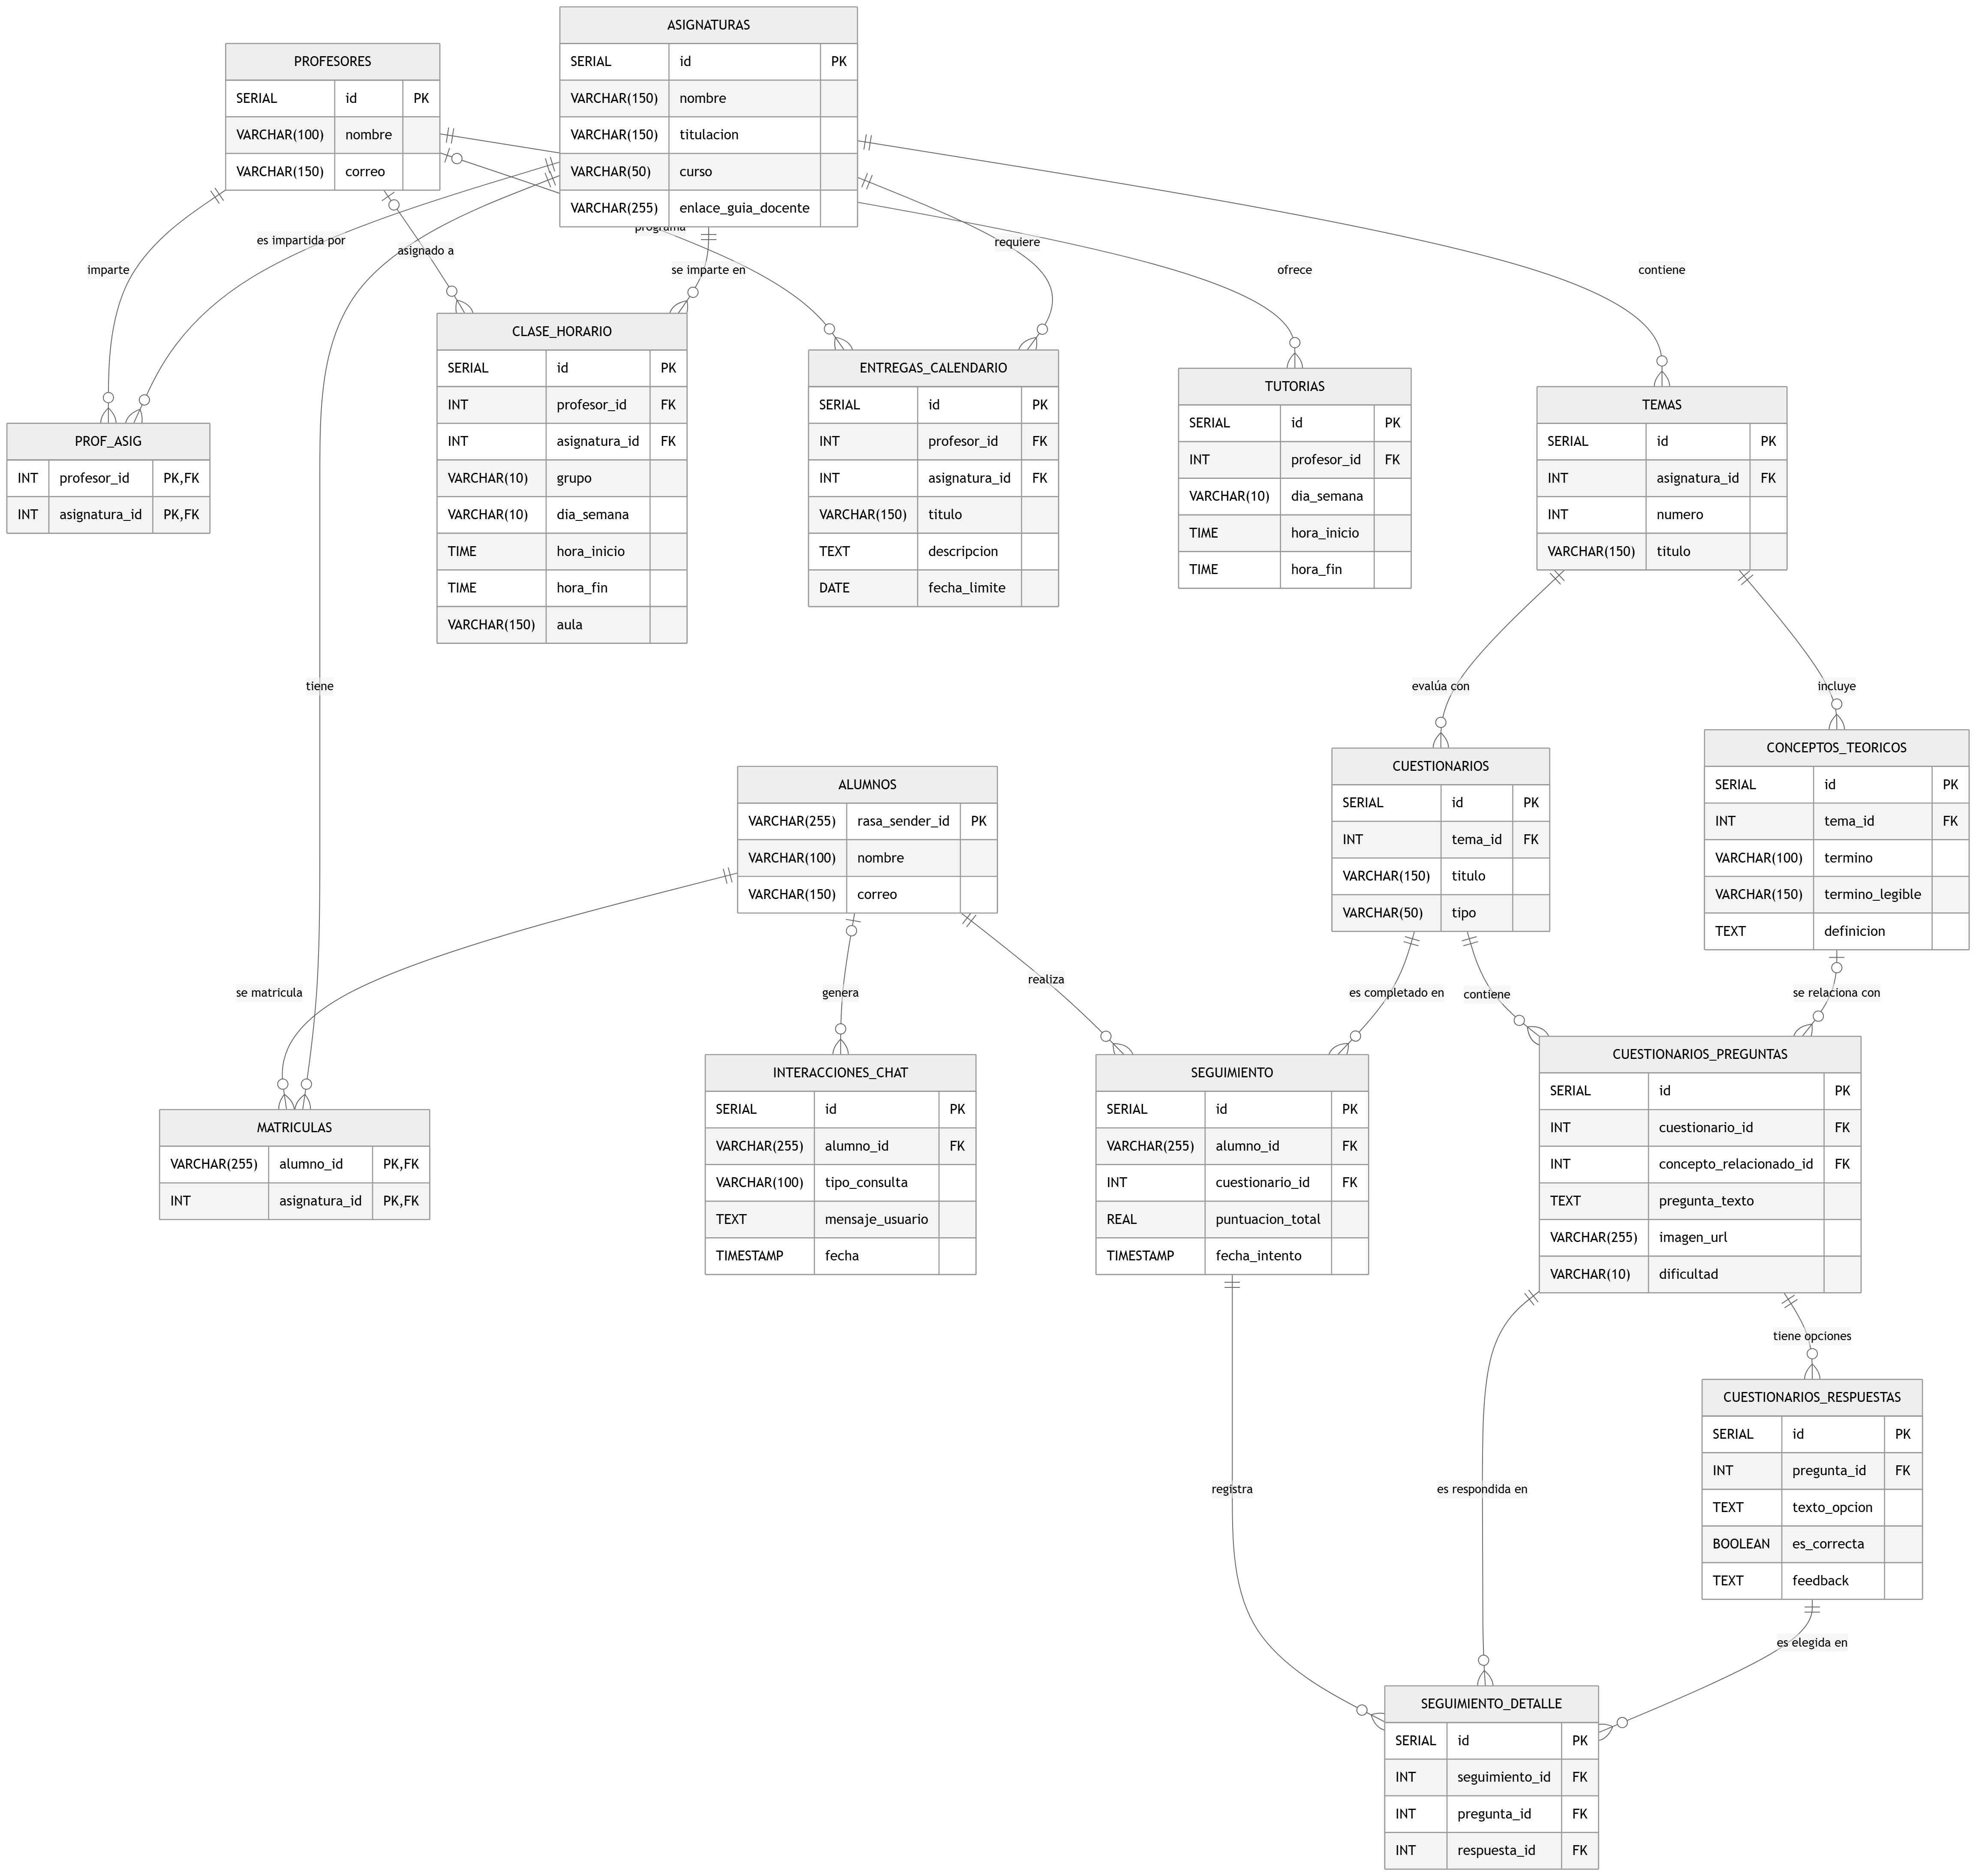
\includegraphics[width=0.9\textwidth]{img/modelo_relacional.png}
    \caption{Diagrama del Modelo Relacional del repositorio educativo y el sistema de seguimiento transaccional.}
    \label{fig:modelo_er}
\end{figure}

A continuación, se detalla el propósito pedagógico y la configuración técnica de los bloques esenciales del esquema relacional:

\subsection{Capa Entidad-Relación Independiente e Informativa}
El nivel primario del esquema lo constituyen las entidades que no albergan dependencias externas y dan soporte de identidad al sistema:
\begin{itemize}
    \item \textbf{\texttt{ALUMNOS}:} Gestiona el censo de usuarios estudiantes del asistente conversacional. Su clave primaria es el campo \texttt{rasa\_sender\_id}, el cual almacena el identificador numérico unívoco proporcionado de forma nativa por la API de Telegram. Esto permite asociar el historial y el contexto de interacción al alumno sin necesidad de credenciales adicionales.
    
    \item \textbf{\texttt{PROFESORES} y \texttt{ASIGNATURAS}:} En el estado actual del asistente, la tabla de profesorado cumple un rol de carácter meramente informativo. Dado que las interacciones del profesor no difieren funcionalmente de las del alumno, el almacenamiento de sus datos responde a la necesidad de resolver dudas administrativas en caliente cuando los alumnos preguntan al chatbot sobre quién imparte la asignatura, sus correos institucionales o sus horarios de tutoría.
\end{itemize}

\subsection{Estructuración del Contenido Educativo Dinámico}
La carga dinámica y personalizada del temario se soporta a través de las relaciones dependientes de la tabla \texttt{TEMAS}. Cuando un estudiante interactúa con el bot solicitando revisar contenidos o realizar evaluaciones, Rasa recopila los temas disponibles y ofrece un abanico dinámico de opciones basado en los registros reales de la base de datos. Esta información se nutre de dos ramas:
\begin{enumerate}
    \item \textbf{Capa de Refuerzo Teórico (\texttt{CONCEPTOS\_TEORICOS}):} Almacena las definiciones conceptuales organizadas por tema. Utiliza campos llave de tipo slug (\texttt{termino}) para el emparejamiento con el motor NLU de Rasa y cadenas descriptivas (\texttt{termino\_legible}) para maquetar la respuesta conversacional final que leerá el alumno.
    
    \item \textbf{Capa de Evaluación y Aprendizaje(\texttt{CUESTIONARIOS}, \texttt{CUESTIONARIOS\_PREGUNTAS} y \texttt{CUESTIONARIOS\_RESPUESTAS}):} Divide las actividades evaluativas según su naturaleza conceptual o práctica. Las preguntas soportan de forma nativa la inclusión de URLs de imágenes (\texttt{imagen\_url}), posibilitando que el bot envíe diagramas o grafos complejos de ejercicios prácticos directamente al chat de Telegram. Por su parte, la tabla de respuestas incluye banderas lógicas (\texttt{es\_correcta}) y campos de \texttt{feedback} personalizados para argumentar el resultado al instante de recibir la pulsación del estudiante.
\end{enumerate}

\subsection{Subsistema de Trazabilidad y Captura de Métricas Adaptativas}
La inteligencia adaptativa del proyecto requiere un registro transaccional meticuloso del desempeño estudiantil, superando la naturaleza efímera de las sesiones de chat convencionales. Para ello se han diseñado las entidades \texttt{SEGUIMIENTO} y \texttt{SEGUIMIENTO\_DETALLE}.\\

A medida que el alumno interactúa respondiendo las preguntas de una prueba práctica o conceptual, el servidor de acciones de Rasa inserta de forma instantánea el acierto, el fallo y la puntuación obtenida en el intento. Este registro pormenorizado cumple una doble función técnica crítica:
\begin{itemize}
    \item \textbf{Cálculo de Calificaciones en Caliente:} Permite al bot recuperar el histórico de intentos del alumno en la sesión activa, calcular su porcentaje de éxito acumulado y moldear el flujo conversacional basándose en su rendimiento del momento.
    
    \item \textbf{Generación del Dataset de Inteligencia:} Estas tablas actúan como la fuente de datos primaria que registra la evolución del aprendizaje del alumno. Los aciertos, errores y estadísticas históricas recopiladas en estas relaciones son las que posteriormente se agregan, estructuran y transforman para alimentar y entrenar el clasificador del Perceptrón Multicapa (MLP) del sistema de recomendación, cerrando de esta forma el bucle de personalización pedagógica.
\end{itemize}

\section{Diseño del Flujo Conversacional (Rasa)}
\label{sec:diseno_conversacional}

El procesamiento del lenguaje natural (NLP) y el control de los hilos de diálogo del asistente adaptativo se articulan mediante el marco de desarrollo \textit{Rasa 3.x}. La ventaja técnica fundamental de este diseño frente a la versión precedente radica en que el diálogo ya no está restringido a reglas rígidas encadenadas a intenciones estáticas. En su lugar, el sistema utiliza un espacio de estado unificado que coordina el modelo NLU, la extracción de entidades y una memoria contextual a corto plazo para manejar dinámicamente las peticiones pedagógicas del alumnado.

\subsection{Modelo NLU: Catálogo de Intenciones y Entidades}
La semántica conversacional del bot se define a partir de un conjunto de intenciones (\textit{intents}) entrenadas para discernir las solicitudes del usuario. Estas intenciones se categorizan en tres bloques funcionales bien diferenciados:
\begin{itemize}
    \item \textbf{Control y Gestión del Flujo:} Comprende intenciones esenciales como el saludo (\texttt{greet}), el inicio (\texttt{start}), la despedida (\texttt{goodbye}), la confirmación (\texttt{affirm}), la negación (\texttt{deny}) o la salida explícita de un cuestionario (\texttt{salir\_cuestionario}).
    \item \textbf{Consultas Administrativas e Informativas:} Engloba las intenciones destinadas a interrogar los metadatos de la asignatura, tales como horarios por días de la semana (\texttt{lunes} a \texttt{viernes}), horarios de teoría o prácticas (\texttt{fechas\_horarios\_teoria}, \texttt{fechas\_horarios\_practica}), profesorado (\texttt{profesorado}), canales de contacto (\texttt{correos\_profesor}), fechas de exámenes (\texttt{entregas}) o noticias (\texttt{noticia}).
    \item \textbf{Interacción Pedagógica y Adaptativa:} Representa el núcleo de la nueva solución, permitiendo al usuario solicitar actividades (\texttt{repasar}, \texttt{conceptos}, \texttt{cuestionarios}, \texttt{ejercicios}), realizar selecciones en caliente (\texttt{seleccionar\_tema}, \texttt{seleccionar\_concepto}, \texttt{seleccionar\_cuestionario}), consultar estadísticas de rendimiento (\texttt{ver\_progreso}) o invocar proactivamente al motor predictivo (\texttt{recomendar}).
\end{itemize}

En paralelo, para extraer parámetros variables inyectados en los mensajes del alumno sin necesidad de fragmentar las intenciones, la canalización NLU extrae cuatro entidades específicas de manera transversal: la etiqueta temática (\texttt{tema\_actual}), el identificador interno del concepto (\texttt{concepto\_id}), la tipología de prueba (\texttt{tipo\_cuestionario}) y el identificador de la prueba seleccionada (\texttt{cuestionario\_id\_seleccionado}).

\subsection{Espacio de Estados y Canales de Contexto (\textit{Slots})}
La capacidad del asistente para recordar la identidad del alumno y determinar qué tema se está evaluando se modela técnicamente mediante \textit{slots}. Estas variables residen en la memoria de la conversación y conservan su valor a lo largo del hilo conversacional. A continuación, se detalla la configuración de las variables de estado críticas del dominio:

\begin{itemize}
    \item \textbf{\texttt{requiere\_registro} y \texttt{matriculado}:} Variables de tipo booleano. El campo \texttt{requiere\_registro} posee la propiedad \texttt{influence\_conversation: true}, lo que significa que altera directamente las políticas de decisión de Rasa para desviar el flujo hacia el formulario de bienvenida si el identificador del alumno no existe en la base de datos relacional.
    \item \textbf{\texttt{nombre} y \texttt{correo}:} Cadenas de texto mapeadas mediante la regla \texttt{from\_text} bajo la condición condicional estricta de encontrarse dentro del ciclo activo del formulario \texttt{registro\_form}.
    \item \textbf{\texttt{tema\_actual}, \texttt{tipo\_cuestionario} y \texttt{cuestionario\_id\_seleccionado}:} Almacenan el contexto de estudio del estudiante, mapeándose directamente desde sus entidades homónimas (\texttt{from\_entity}). Gracias a esto, si el alumno selecciona el "Tema 2", el bot retiene dicho estado en memoria y las peticiones posteriores de cuestionarios o conceptos se filtran automáticamente por ese tema en la base de datos sin necesidad de volver a solicitarlo.
    \item \textbf{\texttt{pregunta\_actual\_idx}, \texttt{aciertos\_cuestionario} y \texttt{seguimiento\_id}:} Variables transaccionales de tipo \texttt{any} manipuladas de forma exclusiva por las acciones personalizadas del \textit{Action Server} mediante mapeos personalizados (\texttt{custom}). Actúan como el índice del bucle evaluativo, el contador de respuestas correctas en caliente y la llave primaria de la sesión de seguimiento insertada, respectivamente.
    \item \textbf{\texttt{respuesta\_generica}:} Variable de texto configurada para capturar cualquier mensaje libre enviado por el estudiante (\texttt{from\_text}) durante la ejecución del bucle evaluativo, con la única restricción de ignorar el comando de salida (\texttt{not\_intent: salir\_cuestionario}).
\end{itemize}

\subsection{Mecanismos de Control Mediante Bucles de Formulario (\textit{Forms})}
Para gestionar interacciones complejas que exigen la recolección secuencial de datos o respuestas, el sistema implementa la abstracción de formularios (\texttt{forms}) de Rasa, delegando la validación en el servidor de acciones:
\begin{enumerate}
    \item \textbf{\texttt{registro\_form}:} Bloquea el hilo de diálogo inicial obligando a capturar de manera secuencial los campos mandatorios \texttt{nombre} y \texttt{correo} antes de habilitar las funciones del chatbot.
    \item \textbf{\texttt{cuestionario\_id\_seleccionado} en el bucle dinámico:} Para resolver el problema de la versión anterior (donde las intenciones de respuesta estaban limitadas y cableadas de forma estática como \texttt{A1} o \texttt{A3}), esta arquitectura utiliza el formulario \texttt{cuestionario\_dinamico\_form}. Este formulario requiere la captura cíclica de la variable \texttt{respuesta\_generica}. En cada iteración, Rasa captura el texto libre introducido por el estudiante (ya sea la letra de la opción o el contenido) y delega la validación de manera dinámica al componente de backend \texttt{validate\_cuestionario\_dinamico\_form}, el cual compara la entrada con la respuesta correcta almacenada en PostgreSQL, calcula el feedback en tiempo de ejecución, limpia el slot del texto e incrementa el índice para la siguiente pregunta de forma totalmente agnóstica al tema bajo evaluación.
\end{enumerate}

\newpage
\section{Diseño de la Lógica de Backend (Action Server)}
\label{sec:diseno_backend}

La lógica de negocio del asistente, la carga de contenidos bajo demanda y la pasarela de persistencia se implementan mediante un servidor de acciones personalizadas (\textit{Action Server}) desarrollado en \textit{Python} utilizando el SDK de Rasa. El núcleo operativo del backend se estructura mediante la librería nativa \texttt{psycopg2}, estableciendo un aislamiento estricto en la gestión de conexiones mediante el uso de gestores de contexto (\texttt{with}) que garantizan la apertura y cierre automático de canales de comunicación con \textit{PostgreSQL} ante excepciones críticas de red.\\

El servidor de acciones se compone de tres módulos lógicos esenciales que operan de manera síncrona con el estado del bot:

\subsection{Control de Seguridad, Registro y Trazabilidad Universal}
Para mitigar el acceso no autorizado a los materiales de estudio, toda acción pedagógica del sistema se antepone a una validación delegada:
\begin{itemize}
    \item \textbf{Verificación de Censo (\texttt{ActionCheckRegistro}):} Interroga la relación \texttt{ALUMNOS} mediante el \texttt{sender\_id} de Telegram. Si el registro no existe, inyecta el valor booleano \texttt{True} en el slot \texttt{requiere\_registro} para disparar la captura de datos mediante \texttt{registro\_form}. En caso de fallas transaccionales, se invoca una directiva \texttt{UserUtteranceReverted} para congelar la conversación y salvaguardar la coherencia del diálogo.
    \item \textbf{Validación de Matrícula (\texttt{ActionCheckMatricula}):} Comprueba en caliente mediante la función \texttt{esta\_matriculado} si el usuario posee un registro activo en la tabla \texttt{MATRICULAS} emparejado con la constante \texttt{ASIGNATURA\_ID\_ACTIVA} (fijada técnicamente en el identificador $1$ para la asignatura de Redes).
    \item \textbf{Auditoría de Conversaciones (\texttt{ActionRegistrarIntent}):} Despacha un log automático en la base de datos registrando el nombre del intent extraído por el clasificador NLU junto a su porcentaje exacto de confianza (\texttt{confidence}) y la cadena original de texto escrita por el alumno.
\end{itemize}

\subsection{Abstracción de Contenidos y Bucle Evaluativo Agnóstico}
El desacoplamiento del material didáctico se implementa a través de las funciones de carga \texttt{load\_conceptos} y \texttt{load\_preguntas}. En el caso de los cuestionarios, la acción \texttt{ActionResetCuestionarioDinamico} instancia una sesión evaluativa llamando a la rutina \texttt{iniciar\_seguimiento}. 

La arquitectura transaccional de respuestas implementa la siguiente lógica de negocio dentro del método de validación \texttt{validate\_respuesta\_generica}:
\begin{enumerate}
    \item El sistema captura el texto libre introducido por el estudiante y realiza un filtrado preventivo mediante la estructura \texttt{ignore\_words} para bloquear la inserción de comandos accidentales de navegación.
    \item Se evalúa la respuesta mediante reglas booleanas de coincidencia de palabras (\texttt{words}) para flexibilizar la corrección (admitiendo tanto la cadena literal como el índice de la opción).
    \item El backend busca el identificador de la opción seleccionada mediante \texttt{get\_respuesta\_id\_elegida} e inserta de forma síncrona el detalle del intento en la tabla \texttt{SEGUIMIENTO\_DETALLE} mediante sentencias \texttt{ON CONFLICT ... DO UPDATE}.
    \item Si se alcanza el final de la lista de preguntas, la acción calcula de forma ponderada la calificación final sobre una escala de diez puntos e invoca la rutina \texttt{actualizar\_puntuacion} en PostgreSQL.
\end{enumerate}

\subsection{Capa de Inteligencia Adaptativa: Integración del Modelo Predictivo MLP}
El motor adaptativo se ejecuta en caliente a través de la clase personalizada \texttt{ActionRecomendar}. Esta clase implementa el puente de unión de ingeniería entre las transacciones almacenadas y la tubería de inferencia del modelo matemático mediante la librería \texttt{joblib}.\\

El flujo de integración y construcción de la predicción sigue un algoritmo matemático secuencial estricto:

\begin{figure}[H]
    \centering
    \scalebox{0.82}{%
        \begin{tikzpicture}[
            startstop/.style={rectangle, rounded corners, draw=epscoscuro, fill=epscoscuro!10, text width=5cm, align=center, minimum height=1.2cm, font=\bfseries\small},
            process/.style={rectangle, draw=epscmedio, fill=epscmedio!10, text width=5cm, align=center, minimum height=1.2cm, font=\small},
            decision/.style={rectangle, rounded corners=0.6cm, draw=epscverde, fill=epscverde!10, text width=3cm, align=center, minimum height=1.2cm, font=\small\bfseries},
            output/.style={rectangle, rounded corners, draw=epscverde, fill=epscverde!5, text width=4.2cm, align=center, minimum height=1.2cm, font=\footnotesize},
            arrow/.style={thick, ->, >=stealth, draw=gray!80}
        ]
            % Nodos
            \node (inicio) [startstop] at (0,0) {1. Alumno solicita\\recomendación};
            \node (db) [process] at (0,-2) {2. Consulta Analítica SQL\\(\texttt{get\_progreso\_alumno})\\Extracción de datos en bruto};
            \node (vector) [process] at (0,-4) {3. Construcción del Vector\\de Características\\(15 Dimensiones / NumPy Array)};
            \node (mlp) [process] at (0,-6) {4. Inferencia Predictiva en caliente\\(\texttt{clf.predict(X)} via \textit{joblib})};
            \node (decidir) [decision] at (0,-8.2) {Evaluación\\de la Salida};
            
            % Salidas
            \node (out_avanzar) [output] at (0,-10.5) {\textbf{avanzar\_siguiente\_tema}\\Invitación motivacional y botón al próximo tema};
            \node (out_repasar) [output] at (-5.5,-10.5) {\textbf{repasar\_tema\_X}\\Aviso académico de refuerzo y botón al tema débil};
            \node (out_global) [output] at (5.5,-10.5) {\textbf{hacer\_examen\_global}\\Mensaje de dominio total. Preparación examen final};

            % Conexiones (Flechas)
            \draw [arrow] (inicio) -- (db);
            \draw [arrow] (db) -- (vector);
            \draw [arrow] (vector) -- (mlp);
            \draw [arrow] (mlp) -- (decidir);
            
            % Rutas de decisión
            \draw [arrow] (decidir.south) -- node[anchor=west] {avanzar} (out_avanzar.north);
            \draw [arrow] (decidir.west) -| node[anchor=south, near start, xshift=-0.5cm] {repasar} (out_repasar.north);
            \draw [arrow] (decidir.east) -| node[anchor=south, near start, xshift=0.5cm] {excelente} (out_global.north);
        \end{tikzpicture}%
    }
    \caption{Flujo técnico de agregación de métricas y tubería de inferencia adaptativa basada en el Perceptrón Multicapa.}
    \label{fig:pipeline_recomendacion}
\end{figure}
\begin{enumerate}
    \item \textbf{Agregación y Extracción Relacional:} El sistema invoca la función analítica \texttt{get\_progreso\_alumno}. Esta rutina procesa el histórico transaccional del alumno y devuelve las métricas unificadas de días de actividad, volumen total de interacciones y número de conceptos consultados.
    \item \textbf{Estructuración del Vector Físico de Características:} Para adecuar los datos relacionales al espacio de entrada multidimensional que exige la red neuronal, el backend genera de manera dinámica un vector de longitud fija conformado por quince características numéricas ($15$ dimensiones) estructurado exactamente bajo la siguiente ecuación lógica:
    \begin{equation}
        V_{features} = [D_{act}, I_{tot}, C_{cons}] \mathbin{\Vert} [Ind_{t1}, \dots, Ind_{t6}] \mathbin{\Vert} [N_{t1}, \dots, N_{t6}]
    \end{equation}
    Donde $D_{act}$ representa los días activos, $I_{tot}$ las interacciones y $C_{cons}$ los conceptos consultados. El bloque $[Ind_{t1 \dots t6}]$ representa indicadores binarios ($0$ o $1$) que marcan si el tema ha sido intentado, mientras que el bloque $[N_{t1 \dots t6}]$ inyecta la calificación máxima real (\textit{float}) obtenida por el alumno para cada uno de los seis temas del plan de estudios.
    \item \textbf{Inferencia Predictiva:} El vector se transforma en una matriz de entrada compatible con \textit{NumPy} (\texttt{np.array([features])}) y se inyecta en caliente en la instancia del clasificador cargado del Perceptrón Multicapa (\texttt{clf.predict(X)}).
    \item \textbf{Alteración Dinámica del Diálogo:} Dependiendo de la cadena de texto devuelta por la inferencia de la red neuronal, el asistente bifurca proactivamente la conversación sin intervención del motor de Rasa:
    \begin{itemize}
        \item Si la salida coincide con el patrón \texttt{repasar\_tema\_X}, el bot maqueta un mensaje de aviso académico sugiriendo reforzar dicha área y adjunta botones interactivos precargados con la carga útil (\textit{payload}) de selección explícita del tema detectado.
        \item Si la salida dictamina \texttt{avanzar\_siguiente\_tema}, el código escanea el vector de indicadores en busca de la primera posición vacía y genera dinámicamente una invitación motivacional apuntando hacia el inicio del nuevo tema.
        \item Si la salida clasifica el estado como \texttt{hacer\_examen\_global}, se informa al estudiante de que ha alcanzado el dominio completo de la asignatura y se encuentra preparado para la prueba de evaluación final presencial.
    \end{itemize}
\end{enumerate}

\chapter{Estudio del Modelo Predictivo}
\label{cap:estudio_modelos}

Con la finalidad de proporcionar al alumno una experiencia pedagógica realmente adaptativa, se ha llevado a cabo un estudio sobre tres modelos de Aprendizaje automático: Árbol de Decisión (\textit{Decision Tree}), Bosque Aleatorio (\textit{Random Forest}) y un Perceptrón Multicapa (\textit{MLP - Red Neuronal}). El objetivo es determinar qué algoritmo ofrece un mayor rendimiento entre la precisión de las recomendaciones y el coste computacional.

\section{Análisis del Conjunto de Datos Sintético}

Para el entrenamiento y evaluación de los modelos, se generó un conjunto de datos sintético de 10.000 muestras, simulando diversas estadísticas del alumnado (días activos, volumen de interacciones, notas en temas superados, etc.).\\

Para certificar que los modelos aprenderían patrones de comportamiento coherentes, se generó la Matriz de Correlación de las características del conjunto de datos (ver Figura \ref{fig:correlation_matrix}).

\begin{figure}[H]
    \centering
    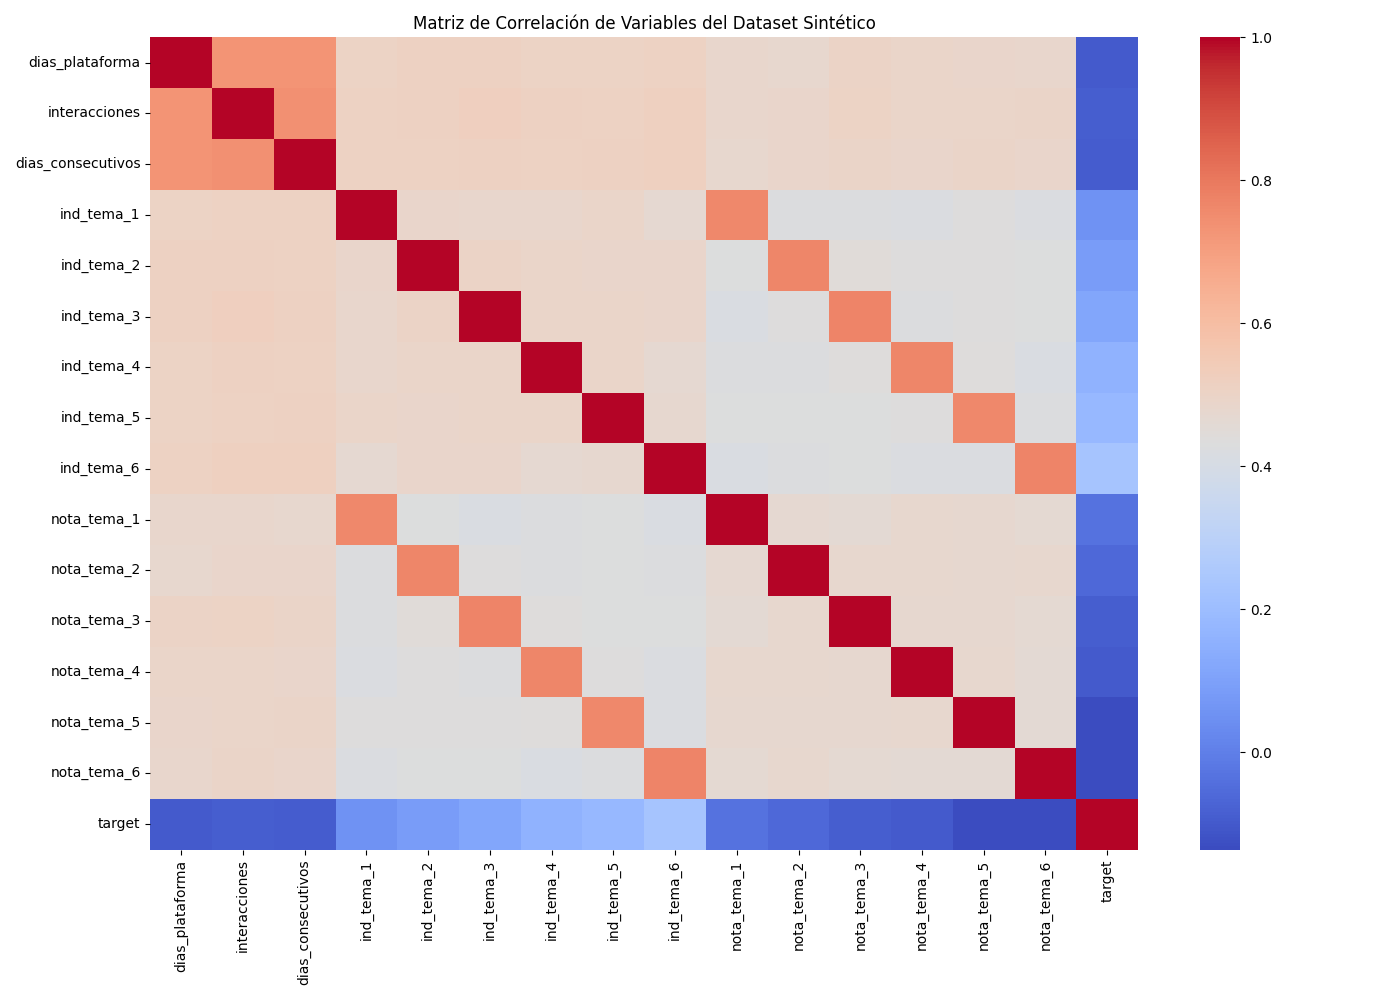
\includegraphics[width=0.85\textwidth]{img/dataset_correlation_matrix.png}
    \caption{Matriz de correlación de las variables del dataset sintético.}
    \label{fig:correlation_matrix}
\end{figure}

El análisis de correlación confirma que los indicadores de temas cursados y sus respectivas calificaciones tienen una correlación lógica respecto a la acción a recomendar, validando así la estructura del conjunto de entrenamiento.

\section{Evaluación y Búsqueda de Hiperparámetros}

Se diseñó una malla de hiperparámetros (\textit{GridSearch}) evaluada con validación cruzada de tres particiones (3-folds) para garantizar que la comparativa fuera justa y todos los modelos operaran con su mejor configuración posible. Las métricas globales obtenidas se resumen gráficamente en las siguientes figuras.

\begin{figure}[htpb]
    \centering
    \begin{minipage}{0.48\textwidth}
        \centering
        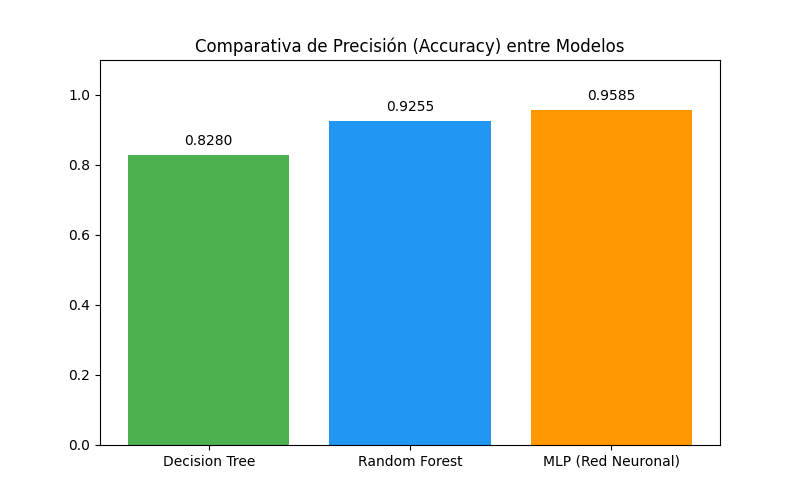
\includegraphics[width=\textwidth]{img/comparativa_accuracy.png}
        \caption{Precisión global por modelo.}
    \end{minipage}\hfill
    \begin{minipage}{0.48\textwidth}
        \centering
        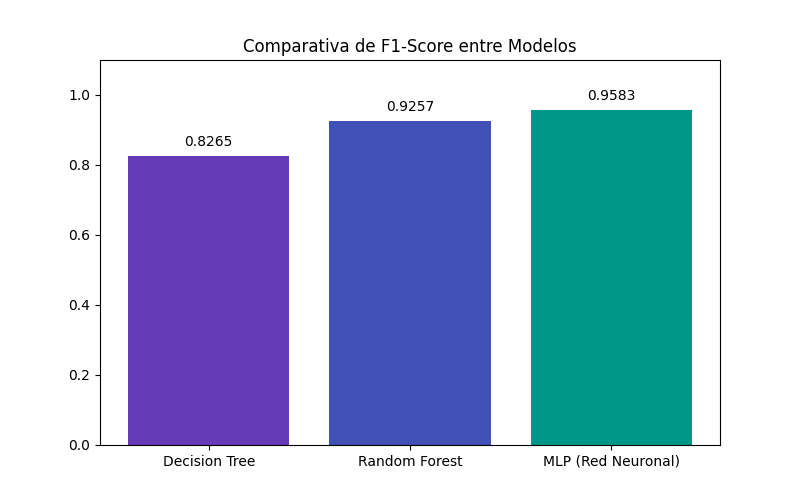
\includegraphics[width=\textwidth]{img/comparativa_f1.png}
        \caption{F1-Score por modelo.}
    \end{minipage}
\end{figure}

Como se observa en los resultados, el \textbf{Perceptrón Multicapa (MLP)} es el modelo más preciso, superando el 95.8\% de \textit{Accuracy} y \textit{F1-Score} con una arquitectura de 32 neuronas ocultas, activación \textit{ReLU} y el optimizador \textit{Adam}. Por otro lado, el Árbol de Decisión apenas ronda el 82\% de precisión debido a su tendencia al sobreajuste o alta simplicidad en fronteras de decisión complejas. Por último, el Random Forest mejora notablemente la clasificación hasta un 92.5\%, pero sigue actuando peor que el MLP.

\subsection{Análisis de Errores mediante Matrices de Confusión}

Para comprender mejor los fallos en la clasificación, se extrajeron las matrices de confusión sobre un conjunto de prueba de 2.000 muestras (ver Figuras \ref{fig:cm_rf} y \ref{fig:cm_mlp}).\\

\begin{figure}[htpb]
    \centering
    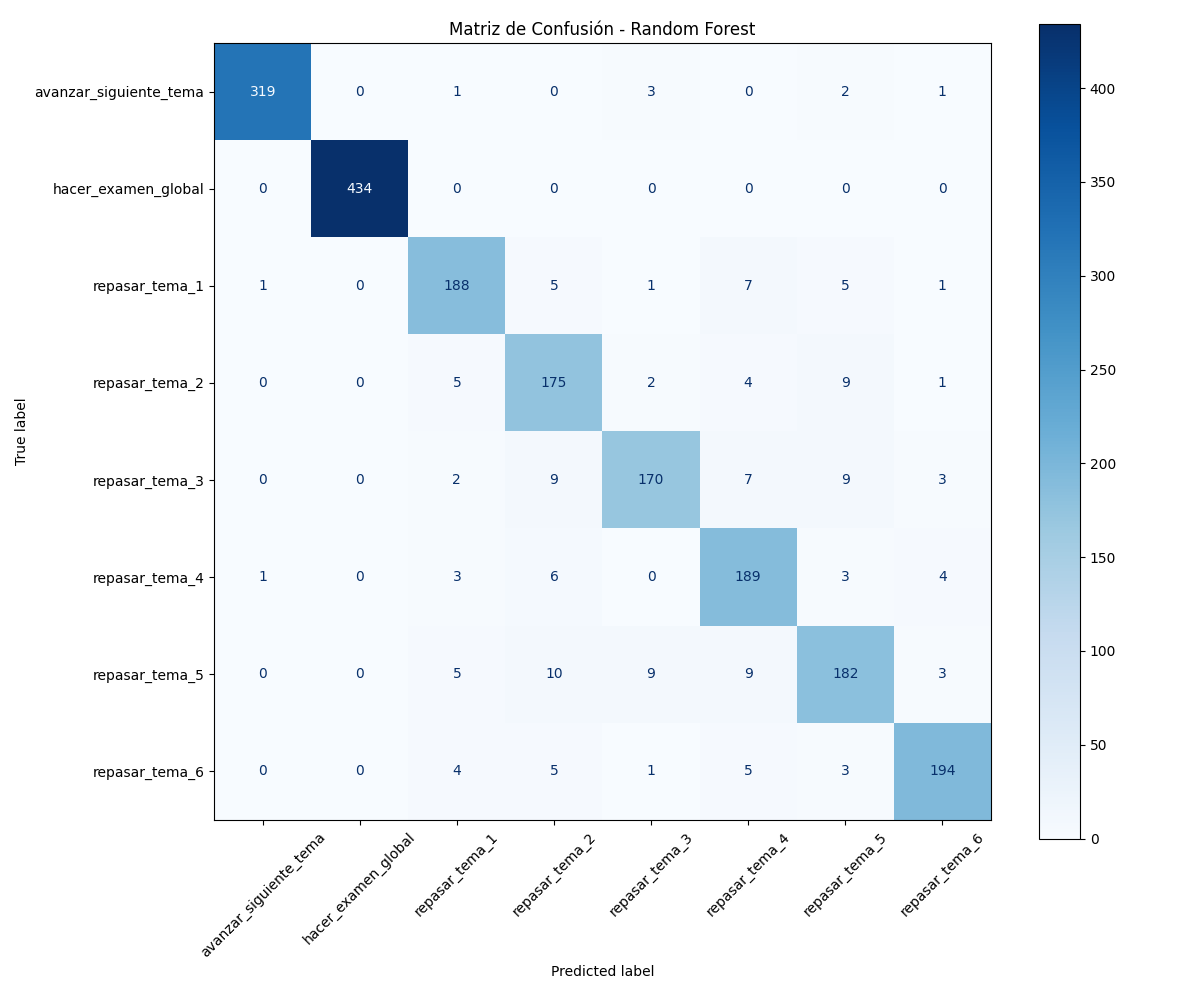
\includegraphics[width=0.8\textwidth]{img/confusion_matrix_random_forest.png}
    \caption{Matriz de confusión del modelo Random Forest.}
    \label{fig:cm_rf}
\end{figure}

\begin{figure}[htpb]
    \centering
    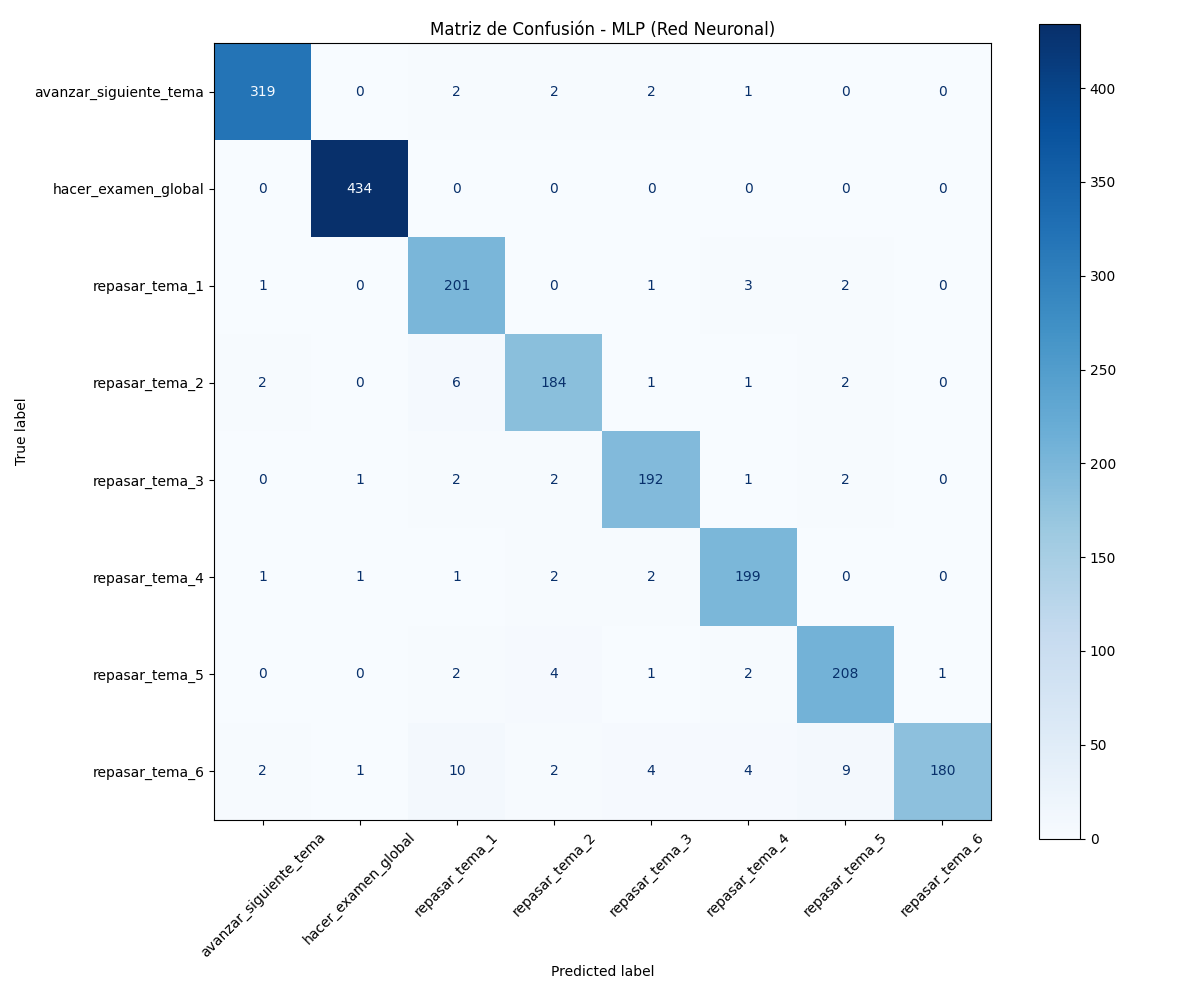
\includegraphics[width=0.8\textwidth]{img/confusion_matrix_mlp_red_neuronal.png}
    \caption{Matriz de confusión del modelo MLP (Red Neuronal).}
    \label{fig:cm_mlp}
\end{figure}

El análisis revela que modelos como el Árbol de Decisión y el Random Forest presentan un mayor grado de confusión entre recomendaciones similares (por ejemplo, confundir repasar el tema 1 con el tema 2), mientras que la Red Neuronal se ajusta mejor a los límites de cuándo el alumno está listo para progresar o cuándo debe volver atrás.

\newpage
\section{Análisis del Coste Temporal y Decisión Final}

En un sistema conversacional en tiempo real, la latencia de respuesta (\textit{tiempo de inferencia}) es un factor crítico. Se midieron tanto los tiempos de ajuste (GridSearch total) como los tiempos de inferencia sobre el conjunto de prueba (2.000 muestras).

\begin{figure}[htpb]
    \centering
    \begin{minipage}{0.48\textwidth}
        \centering
        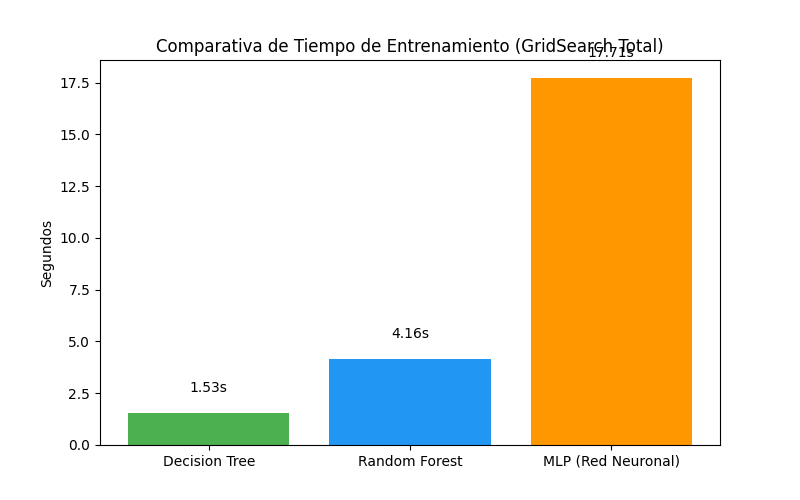
\includegraphics[width=\textwidth]{img/comparativa_tiempo_fit.png}
        \caption{Tiempos de entrenamiento.}
    \end{minipage}\hfill
    \begin{minipage}{0.48\textwidth}
        \centering
        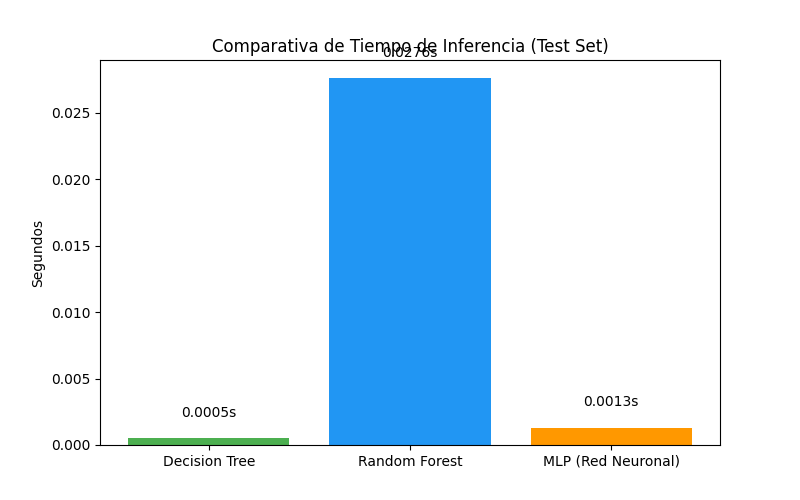
\includegraphics[width=\textwidth]{img/comparativa_tiempo_predict.png}
        \caption{Tiempos de inferencia.}
    \end{minipage}
\end{figure}

El Perceptrón Multicapa requiere un coste computacional significativamente mayor en la fase de entrenamiento (más de 17 segundos frente a los 4 segundos del Random Forest). Sin embargo, este proceso se realiza fuera de la interacción con el alumno, por lo que no penaliza la experiencia del alumno a la hora de conversar con el asistente. En la fase de inferencia (cuando el estudiante solicita la recomendación), el MLP es el más eficiente, requiriendo apenas milisegundos para clasificar las 2.000 peticiones.

\paragraph{Justificación de la elección:} Dados los resultados, el Perceptrón Multicapa (MLP) es seleccionado como el motor de recomendación para el asistente. Su notable superioridad en la precisión de clasificación (95.85\%) combinada con una latencia de inferencia imperceptible para el usuario garantizan un apoyo adaptativo preciso, dinámico y fluido.

\chapter{Conclusiones}
Resumen de los principales logros obtenidos en el trabajo y/o sugerencias sobre posibles futuras mejoras a realizar sobre la solución aportada.

\backmatter

%------------- Bibliografía --------------
\printbibliography
\end{document}

\end{document}
